\documentclass[14pt,a4paper]{extarticle}
\usepackage[T1]{fontenc}
\usepackage[utf8]{inputenc}
\usepackage[scaled]{helvet}
\renewcommand{\familydefault}{\sfdefault}
\usepackage{amsmath}
\usepackage{sansmath}
\sansmath
\usepackage[a4paper,margin=2cm]{geometry}
\usepackage{tikz}
\pagestyle{empty}
% Zweite Seite: 5-mm-Kästchen, 1 cm Rand
\newcommand{\kaestchen}{\newpage\null\begin{tikzpicture}[remember picture,overlay]
\begin{scope}[shift={(current page.south west)}]\draw[step=5mm, black!45, line width=0.3pt] (1cm,1cm) grid (20cm,28.5cm);\draw[black!45, line width=0.3pt] (1cm,1cm) rectangle (20cm,28.5cm);\end{scope}
\end{tikzpicture}}
\setlength{\parindent}{0pt}
\hyphenpenalty=10000

% Kreuzung zweier Geraden. Graue Winkel als Liste Start/Ende/Farbe/Name.
\newcommand{\kreuzung}[1]{%
\begin{tikzpicture}[scale=1.45]
  \foreach \a/\b/\c/\n in {#1} {
    \fill[\c] (0,0) -- (\a:0.85) arc (\a:\b:0.85) -- cycle;
    \node at ({(\a+\b)/2}:1.18) {\large$\n$};
  }
  \draw[thick] (-2.3,0) -- (2.3,0);
  \draw[thick] (230:1.75) -- (50:1.75);
  \fill (0,0) circle (1.6pt);
\end{tikzpicture}}

% Merkblock: Begriff und Text links, Zeichnung rechts.
\newcommand{\block}[3]{%
\begin{minipage}[c]{0.5\textwidth}\raggedright{\Large\bfseries #1\par}\medskip #2\end{minipage}\hfill
\begin{minipage}[c]{0.47\textwidth}\centering #3\end{minipage}\par}

\begin{document}

{\LARGE\bfseries Winkel an Geradenkreuzungen\par}
\vspace{0.7cm}

\block{Voller Kreis und Gerade}{%
Ein voller Kreis hat $360^\circ$.\par\smallskip
Eine Gerade teilt den Kreis in zwei Hälften. Jede Hälfte hat $180^\circ$.}{%
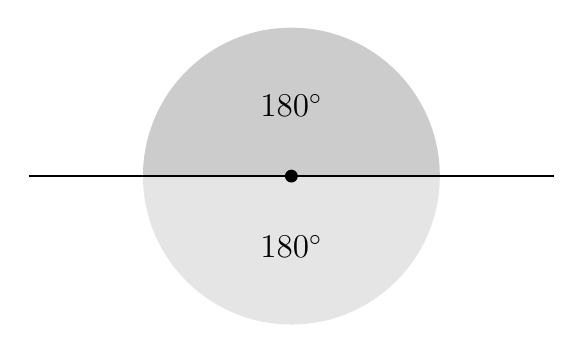
\begin{tikzpicture}[scale=1.45]
  \fill[gray!40] (0,0) -- (1.3,0) arc (0:180:1.3) -- cycle;
  \fill[gray!20] (0,0) -- (-1.3,0) arc (180:360:1.3) -- cycle;
  \draw[thick] (-2.3,0) -- (2.3,0);
  \fill (0,0) circle (1.6pt);
  \node at (0,0.62) {\large$180^\circ$};
  \node at (0,-0.62) {\large$180^\circ$};
\end{tikzpicture}}

\vspace{0.7cm}

\block{Nebenwinkel}{%
Nebenwinkel liegen nebeneinander an einer Geraden. Zusammen sind sie $180^\circ$ groß.
\[
\begin{array}{r@{\;=\;}l@{\qquad}l}
\alpha + \beta & 180^\circ & \mid -\alpha\\[2pt]
\beta & 180^\circ - \alpha &
\end{array}
\]
Beispiel: $\alpha = 35^\circ$\par\smallskip
$\beta = 180^\circ - 35^\circ = 145^\circ$}{%
\kreuzung{0/50/gray!40/\alpha, 50/180/gray!20/\beta}}

\vspace{0.7cm}

\block{Scheitelwinkel}{%
Scheitelwinkel liegen sich an der Kreuzung gegenüber. Sie sind gleich groß.
\[\alpha = \gamma \qquad \beta = \delta\]}{%
\kreuzung{0/50/gray!40/\alpha, 50/180/gray!20/\beta, 180/230/gray!40/\gamma, 230/360/gray!20/\delta}}

\vspace{0.7cm}

% Beispielaufgabe abgesetzt im Rahmen, mit eigener Zeichnung samt Werten
\noindent\fcolorbox{black!50}{white}{\begin{minipage}{\dimexpr\textwidth-2\fboxsep-2\fboxrule\relax}
{\Large\bfseries Beispiel:\ Alle vier Winkel berechnen\par}\smallskip
\begin{minipage}[c]{0.56\linewidth}\raggedright
Kennst du einen Winkel, kannst du alle vier berechnen. Gegeben ist $\alpha = 35^\circ$.\par\medskip
\begin{tabular}{@{}ll@{}}
$\gamma = \alpha = 35^\circ$ & Scheitelwinkel\\[2pt]
$\beta = 180^\circ - 35^\circ = 145^\circ$ & Nebenwinkel\\[2pt]
$\delta = \beta = 145^\circ$ & Scheitelwinkel
\end{tabular}
\end{minipage}\hfill
\begin{minipage}[c]{0.42\linewidth}\centering
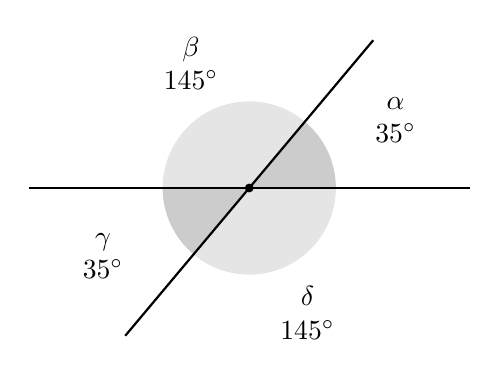
\begin{tikzpicture}
  \fill[gray!40] (0,0) -- (1.1,0) arc (0:50:1.1) -- cycle;
  \fill[gray!20] (0,0) -- (50:1.1) arc (50:180:1.1) -- cycle;
  \fill[gray!40] (0,0) -- (-1.1,0) arc (180:230:1.1) -- cycle;
  \fill[gray!20] (0,0) -- (230:1.1) arc (230:360:1.1) -- cycle;
  \draw[thick] (-2.8,0) -- (2.8,0);
  \draw[thick] (230:2.45) -- (50:2.45);
  \fill (0,0) circle (1.6pt);
  \node[align=center] at (25:2.05) {$\alpha$\\$35^\circ$};
  \node[align=center] at (115:1.75) {$\beta$\\$145^\circ$};
  \node[align=center] at (205:2.05) {$\gamma$\\$35^\circ$};
  \node[align=center] at (295:1.75) {$\delta$\\$145^\circ$};
\end{tikzpicture}
\end{minipage}
\end{minipage}}

\vspace{0.7cm}

{\Large\bfseries Aufgaben im Heft\par}
\medskip
Buch S.\,49 Nr.\,2, 3, 4, 5\par\smallskip
Buch S.\,50 Nr.\,1, 2, 3

\kaestchen
\end{document}
